\documentclass{article}
\usepackage{graphicx}
\usepackage[utf8]{inputenc}
\usepackage{polski}
\usepackage{float}

\author{Kacper Haczkiewicz, Maria Kwintal, Laura Nowak, Paweł Nowak}
\title{\textbf{Projekt zaliczeniowy - dokumentacja}}
\date{Styczeń 2024}

\begin{document}
	
	\maketitle
	
	\section{Wstęp}
	
	\section{Spisu użytych technologii}
	
	\section{Pliki}
	
	\section{Schemat bazy danych}
	
	\subsection{Graficzny schemat bazy}
	
	Poniżej znajduje się graficzny schemat bazy danych.
	
	\begin{figure}[H]
		\centering
		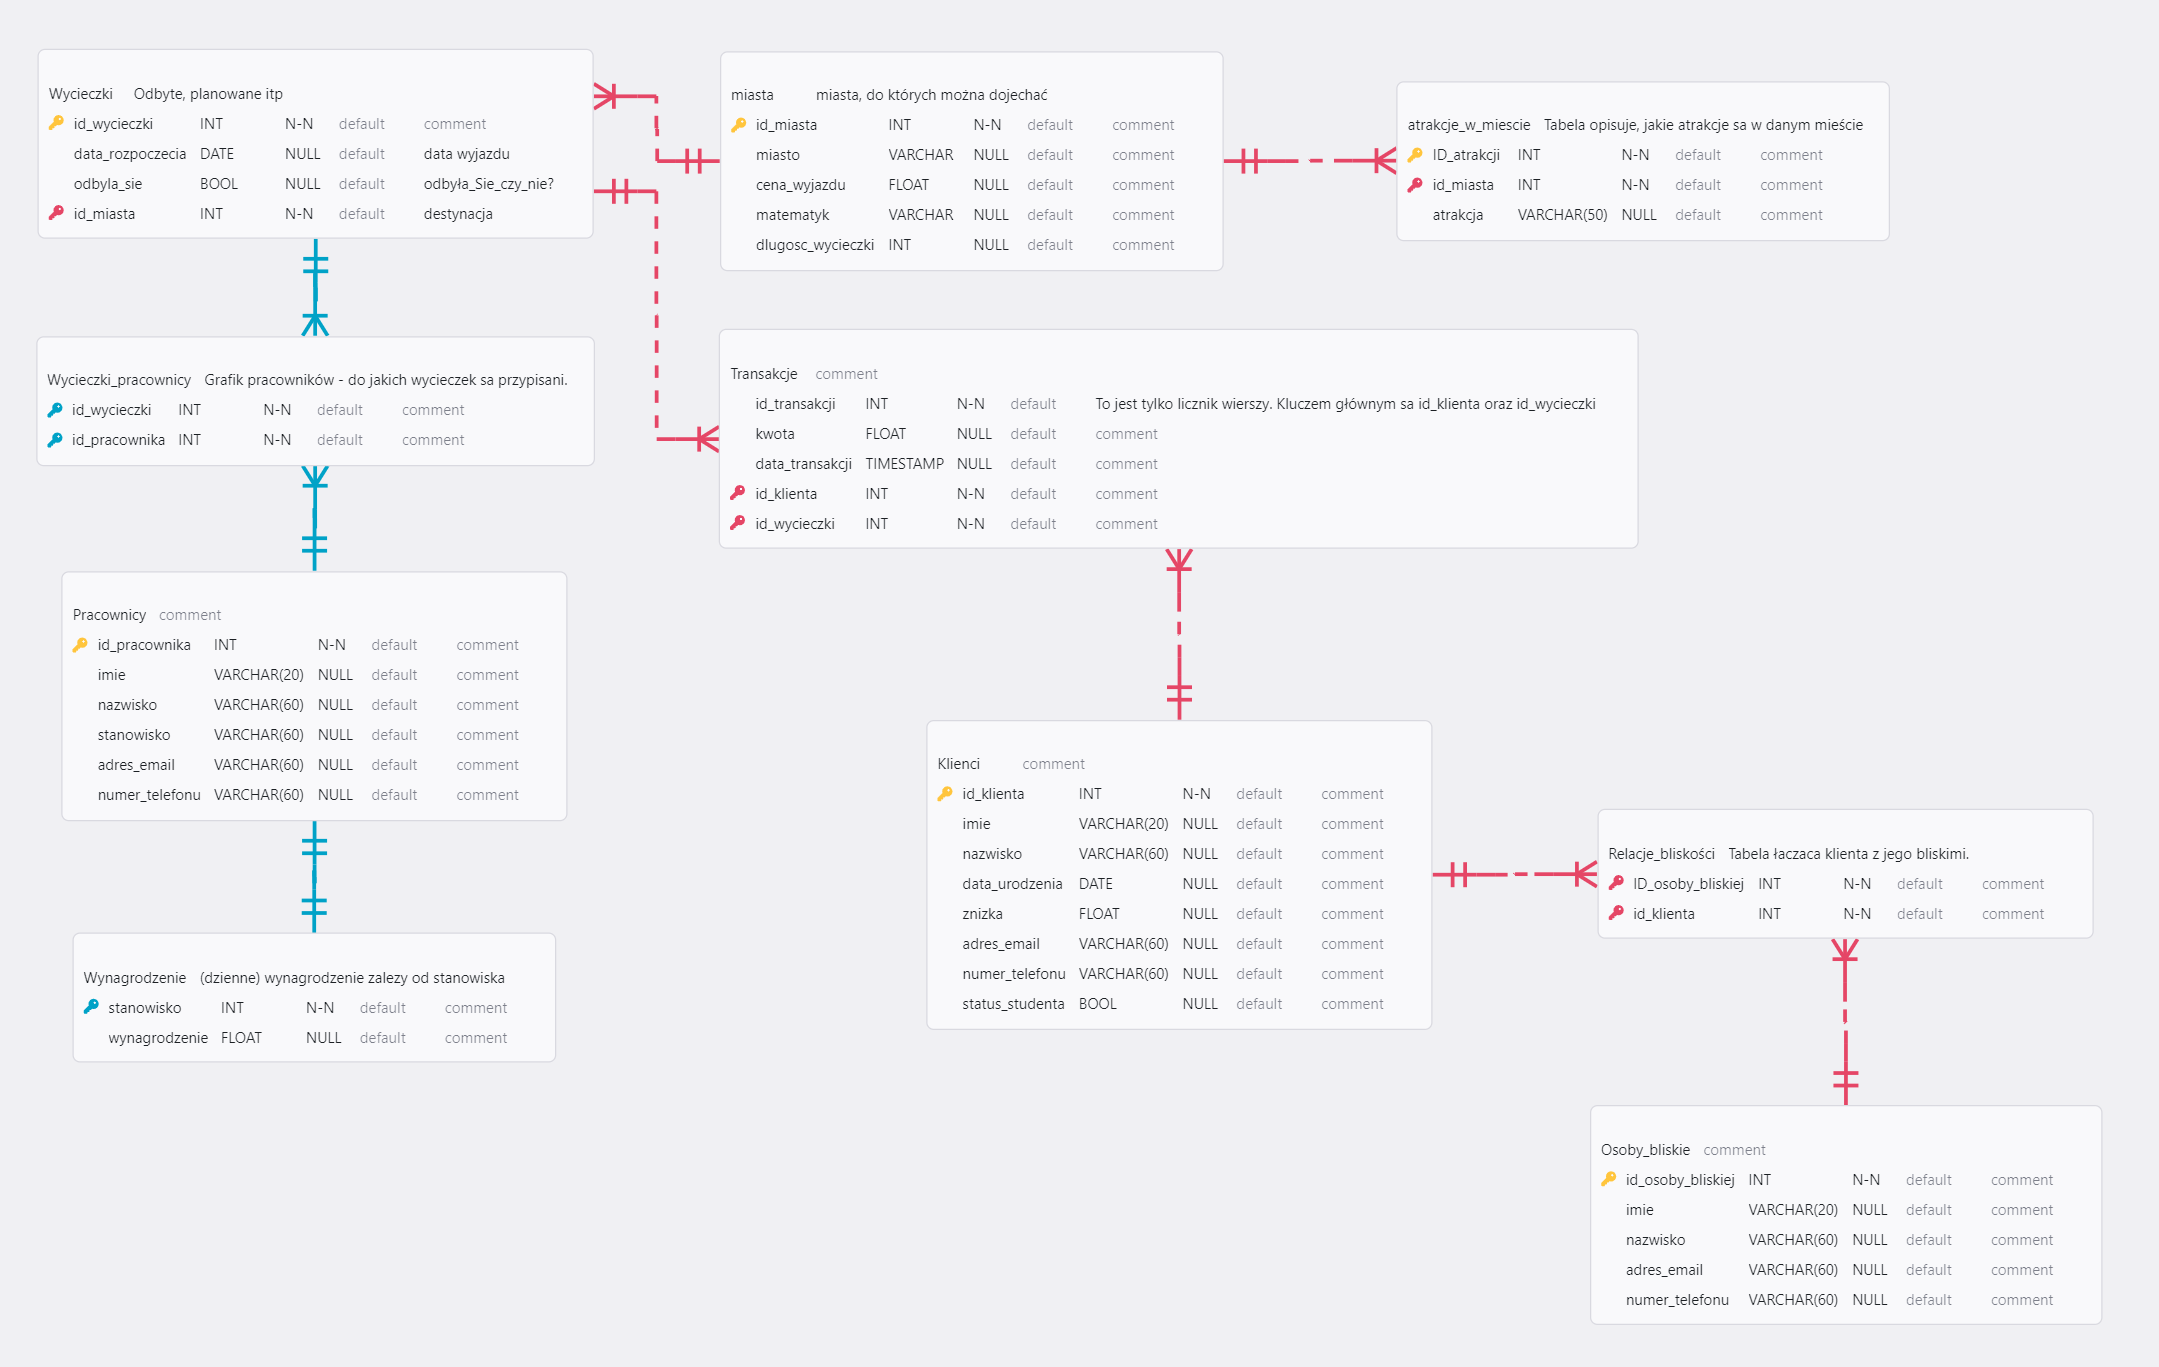
\includegraphics[scale=0.2]{diagram.PNG}
		\caption{Schemat bazy}
	\end{figure}
	
	\subsection{Opis tabel}
	
	Baza danych składa się z niżej opisanych tabel. 
	
	\begin{enumerate}
		\item Klienci
		\begin{itemize}
			\item Atrybuty: id\textunderscore klienta (klucz główny), imie, nazwisko, data\textunderscore urodzenia, znizka, adres\textunderscore email, numer\textunderscore telefonu, status\textunderscore studenta.
			\item Zależności funkcyjne: id\textunderscore klienta → imie, nazwisko, data\textunderscore urodzenia, znizka, adres\textunderscore email, numer\textunderscore telefonu, status\textunderscore studenta.
		\end{itemize}
		
		\item Miasta
		\begin{itemize}
			\item Atrybuty: id\textunderscore miasta (klucz główny), miasto, cena\textunderscore wyjazdu, matematyk, dlugosc\textunderscore wycieczki.
			\item Zależności funkcyjne: id\textunderscore miasta → miasto, cena\textunderscore wyjazdu, matematyk, dlugosc\textunderscore wycieczki.
		\end{itemize}
		
		\item Atrakcje\textunderscore w\textunderscore miescie
		\begin{itemize}
			\item Atrybuty: id\textunderscore atrakcji (klucz główny), atrakcja, id\textunderscore miasta (klucz obcy).
			\item Zależności funkcyjne: id\textunderscore atrakcji → atrakcja, id\textunderscore miasta.
		\end{itemize}
		
		\item Osoby\textunderscore bliskie
		\begin{itemize}
			\item Atrybuty: id\textunderscore osoby\textunderscore bliskiej (klucz główny), imie, nazwisko, adres\textunderscore email, numer\textunderscore telefonu.
			\item Zależności funkcyjne: id\textunderscore osoby\textunderscore bliskiej → imie, nazwisko, adres\textunderscore email, numer\textunderscore telefonu.
		\end{itemize}
		
		\item Relacje\textunderscore bliskosci
		\begin{itemize}
			\item Atrybuty: id\textunderscore osoby\textunderscore bliskiej (część klucza głównego), id\textunderscore klienta (część klucza głównego).
		\end{itemize}
		
		\item Transakcje
		\begin{itemize}
			\item Atrybuty: id\textunderscore transakcji (klucz główny), kwota, data\textunderscore transakcji, id\textunderscore klienta (klucz obcy), id\textunderscore wycieczki (klucz obcy).
			\item Zależności funkcyjne: id\textunderscore transakcji → kwota, data\textunderscore transakcji, id\textunderscore klienta (klucz obcy), id\textunderscore wycieczki (klucz obcy).
		\end{itemize}
		
		\item Wycieczki
		\begin{itemize}
			\item Atrybuty: id\textunderscore wycieczki (klucz główny), data\textunderscore rozpoczecia, odbyla\textunderscore sie, id\textunderscore miasta (klucz obcy).
			\item Zależności funkcyjne: id\textunderscore wycieczki → data\textunderscore rozpoczecia, odbyla\textunderscore sie, id\textunderscore miasta (klucz obcy).
		\end{itemize}
		
		\item Wycieczki\textunderscore pracownicy
		\begin{itemize}
			\item Atrybuty: id\textunderscore wycieczki (część klucza głównego, klucz obcy), id\textunderscore pracownika (część klucza głównego, klucz obcy).
		\end{itemize}
		
		\item Pracownicy
		\begin{itemize}
			\item Atrybuty: id\textunderscore pracownika (klucz główny), imie, nazwisko, stanowisko (klucz obcy), adres\textunderscore email, numer\textunderscore telefonu.
			\item Zależności funkcyjne: id\textunderscore pracownika → imie, nazwisko, stanowisko (klucz obcy), adres\textunderscore email, numer\textunderscore telefonu.
		\end{itemize}
		
		\item Wynagrodzenie
		\begin{itemize}
			\item Atrybuty: stanowisko (klucz główny), wynagrodzenie.
			\item Zależności funkcyjne: stanowisko → wynagrodzenie.
		\end{itemize}
	\end{enumerate}
	
	\subsection{Opis relacji}
	
	Pomiędzy tabelami występują następujące relacje.
	
	\begin{enumerate}
		\item Wycieczki i Wycieczki\textunderscore pracownicy: relacja 1:n - każdy pracownik może być przypisany do wielu wycieczek. Klucz główny tabeli Wycieczki (id\textunderscore wycieczki) występuje jako część klucza głównego w tabeli Wycieczki\textunderscore pracownicy. 
		\item Wycieczki\textunderscore pracownicy i Pracownicy: relacja 1:n - każda wycieczka może mieć wielu pracowników. Klucz główny tabeli Pracownicy (id\textunderscore pracownika) występuje jako część klucza głównego w tabeli Wycieczki\textunderscore pracownicy.
		\item Pracownicy i Wynagrodzenie: relacja 1:1 - jeden pracownik może mieć jedno wynagrodzenie. Klucz główny tabeli Wynagrodzenie (stanowisko) występuje jako klucz obcy w tabeli Pracownicy.
		\item Wycieczki i Miasta: relacja 1:n - wiele wycieczek może odbywać się w jednym mieście. Klucz główny tabeli Miasta (id\textunderscore miasta) jest kluczem obcym w tabeli Wycieczki.
		\item Miasta i Atrakcje\textunderscore w\textunderscore miescie: relacja 1:n - w jednym mieście może być wiele atrakcji. Klucz główny tabeli Miasta (id\textunderscore miasta) jest kluczem obcym w tabeli Atrakcje\textunderscore w\textunderscore miescie.
		\item Wycieczki i Transakcje: relacja 1:n - każda wycieczka może być związana z wieloma transakcjami. Klucz główny tabeli Wycieczki (id\textunderscore wycieczki) występuje jako klucz obcy w tabeli Transakcje.
		\item Transakcje i Klienci: relacja 1:n - jeden klient może być związany z wieloma transakcjami. Klucz główny tabeli Klienci (id\textunderscore klienta) występuje jako klucz obcy w tabeli Transakcje.
		\item Klienci i Relacje\textunderscore bliskosci: relacja 1:n - jeden klient może mieć wiele przypisanych relacji z osobami bliskimi. Klucz główny tabeli Klienci (id\textunderscore klienta) występuje jako klucz obcy w tabeli Relacje\textunderscore bliskosci.
		\item Relacje\textunderscore bliskosci i Osoby\textunderscore bliskie: relacja 1:n - jedna osoba bliska może być powiązana z wieloma klientami. Klucz główny tabeli Osoby\textunderscore bliskie (id\textunderscore osoby\textunderscore bliskiej) występuje jako klucz obcy w tabeli Relacje\textunderscore bliskosci.
	\end{enumerate}
	
	\subsection{Uzasadnienie, że baza jest w EKNF}
	
	
	
	
	\section{Podsumowanie projektu}
	
\end{document}